% LaTeX script for Semester und Diploma Thesis
% Martin Geidl, April 2004
% Edited by Theodor Borsche, April 2015
% This template can be compiled with pdflatex or traditional latex
% If used with pdflatex all images have to be in pdf format

\documentclass[a4paper,11pt,twoside,onecolumn]{book}

% encoding of the input file. If your computer/ editor uses utf8, change the option
\usepackage[latin1]{inputenc}

% language packages for hyphenation, etc
\usepackage[german,english]{babel}
\usepackage{ae} % some additional fonts / symbols


% packages for MATH input
\usepackage{amstext,amssymb,amsbsy,amsmath}
\interdisplaylinepenalty=2500
\usepackage{mathtools} % additional symbols and fixes


% packages for TABLES
%\usepackage{rotating}
\usepackage{booktabs} % for tables, use booktabs. See documentation.
\usepackage{floatrow}
\floatsetup[table]{capposition=top} % ensure caption is above table
\usepackage{lscape} % allows to rotate tables
\usepackage{multirow} % allows to use cells spanning multiple rows

\usepackage{url} % allows to typeset url's with line-breaks
\usepackage[ruled,vlined]{algorithm2e} % for typesetting algorithms


% for UNITS, use siunitx
\usepackage[detect-all, per-mode = fraction]{siunitx}


% GRAPHICS packages
\usepackage{graphicx} % for including figures with \includegraphics[graphicx keys]{file}
\graphicspath{{Figures/}} % you can put figures in this path
\DeclareGraphicsExtensions{.pdf,.png,.jpeg,.eps} % you do not need to type these extensions for figure files
% \usepackage{epstopdf} % convert eps to pdf. Requires ghostscript

\usepackage{float} % additional float definitions and control


% adjust FLOAT placement
\renewcommand{\textfraction}{0.15} % minimum amount of text on a page
\renewcommand{\topfraction}{0.85} % maximum amount a figure at top may use
\renewcommand{\bottomfraction}{0.6} % maximum amount a figure at bottom may use
\renewcommand{\floatpagefraction}{0.55} % minimum amount a figure on its own page must use
\setcounter{totalnumber}{4} % maximum number of figures per page
\setcounter{topnumber}{3} % maximum number of figures at top
\setcounter{bottomnumber}{2} % amximum number of figures at bottom

% COLOR
\usepackage[dvipsnames]{xcolor} % xcolor allows to define colors
% the 10 standard ETH colors in CMYK colorspace
\definecolorset{cmyk}{}{}{%
    eth1, 1,    0.7,  0,   0.30;%
    eth2, 0.75, 0.4,  1,   0.40;%
    eth3, 1,    0.5,  0,   0;%
    eth4, 0.3,  0,    1,   0.55;%
    eth5, 0.2,  1,    0,   0.20;%
    eth6, 0,    0,    0,   0.7;%
    eth7, 0,    0.9,  0.8, 0.20;%
    eth8, 1,    0.25, 0.3, 0.1;%
    eth9, 0,    0.55, 1,   0.40;%
    eth10,0.6,  0,    1,   0 }

% RGB colors don't look as good, use CMYK if possible
\definecolorset{RGB}{}{}{%
    eth1rgb,  31,  64, 122;%
    eth2rgb,  72,  90,  44;%
    eth3rgb,  18, 105, 176;%
    eth4rgb, 114, 121,  28;%
    eth5rgb, 145,   5, 106;%
    eth6rgb, 111, 111, 100;%
    eth7rgb, 168,  50,  45;%
    eth8rgb,   0, 122, 150;%
    eth9rgb, 149,  96,  19;%
    eth10rgb,140, 182,  60} % define ETH corporate design colors. Names are 'eth3', ..., 'eth9'


\selectlanguage{english} % choose language for hyphenation and dates

% \makeatletter
% \newcommand*{\rom}[1]{\expandafter\@slowromancap\romannumeral #1@}
% \makeatother


% correct bad hyphenation here
\hyphenation{op-tical net-works semi-conduc-tor}

\begin{document}
\frontmatter

% Enter your data in the file titlepage.tex
\begin{titlepage}
\begin{center}


\includegraphics[height=12mm]{Figures/eth_logo_lang_pos}
\hfill
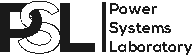
\includegraphics[height=8mm]{Figures/PSL_logo}

\vspace{30mm} Xingliang Fang \\
\vspace{10mm} \textbf{\LARGE Opportunities and requirements for small-to-medium scale energy flexibility management solutions in various power market regimes} \\
\vspace{10mm} Master Thesis \\ PSL1226


\vfill

EEH -- Power Systems Laboratory, ETH Zurich \\
Corporate Strategy Office , Landis+Gyr

\vspace{5mm}

Examiner: Prof.~Dr.~Gabriela Hug \\
Supervisor: Dr.~Donnacha Daly (Landis+Gyr), Jun Xing Chin


\vspace{5mm} Zurich, \today

\end{center}
\end{titlepage}



\chapter*{Abstract}
%\input{abstract}
\newpage


\chapter*{Acknowledgements}
%\input{preface}
\newpage


\tableofcontents
\newpage



% If you use a lot of special acronyms a normal\frac{}{} power engineer doesn't know,
% please explain them here.
\chapter*{List of Acronyms}
\addcontentsline{toc}{chapter}{List of Acronyms}
%\input{acronyms}
% If you are also using lots of equations and symbols, define them in a list of symbols.

\chapter*{List of Symbols}
\addcontentsline{toc}{chapter}{List of Symbols}
%\input{symbols}




\mainmatter

\chapter{Introduction}
%\input{introduction}

%
\chapter{Model Decription}
\label{ch:model}
%\input{control}
\section{Input Model}
\subsection{Renewable}

\section{Optimization}
\subsection{Objective Function}

\begin{equation*}
\begin{aligned}
& \underset{d_t^{DA}, c_t^{DA}, d_t^{RT}, c_T^{RT}, r_t}{\text{maximize}}
& & \sum_t^{t \in T} \mathrm{Revenue_t} \\
& & &= [p_t^{DA} (d_t^{DA}-c_t^{DA}) + p_t^{RT} (d_t^{RT}-c_t^{RT}) + (p_t^r+p_t^{RU} \delta_t^{RU}-p_t^{RD} \delta_t^{RD}) r_t] \Delta t \\
\end{aligned}
\end{equation*}


\textbf{Aggregators/ Neural Traders} - Arbitrage
\begin{equation*}
\begin{aligned}
&Revenue_t \\
& & = p_t * (d_t-c_t) * \Delta t
\end{aligned}
\end{equation*}

\textbf{Generators}  - Increased revenue
\begin{equation*}
\begin{aligned}
&Revenue_t \\
& & = [p_t * (g_t+d_t-c_t) - p_t*g_t]* \Delta t \\
& & = p_t * (d_t-c_t) * \Delta t
\end{aligned}
\end{equation*}

\textbf{Retailer} - Reduced cost
\begin{equation*}
\begin{aligned}
&Revenue_t \\
& & = [p_t*l_t - p_t * (l_t-d_t+c_t) ]* \Delta t \\
& & = p_t * (d_t-c_t) * \Delta t
\end{aligned}
\end{equation*}

\subsection{Constraints}
\textbf{Energy Storage Systems (ES)}
\begin{equation*}
\begin{aligned}
\text{subject to} &  \\
& S_t = \eta_s S_{t-1} + [\eta_c(c_t^{DA}+c_t^{RT}+\delta^{RD}_t r_t)  - \eta_d(d_t^{DA}+d_t^{RT}+\delta^{RU}_t r_t)]\Delta t  \\
& d_t^{DA} + d_t^{RT} +\delta^{RU}_t r_t \leq d_t^{max} \\
& c_t^{DA} + c_t^{RT} +\delta^{RD}_t r_t \leq c_t^{max} \\
& \delta_r r_t \Delta t \leq S_t \leq S_t^{max} - \delta_r r_t \Delta t \\
& d_t^{DA}, c_t^{DA}, d_t^{RT}, c_T^{RT}, r_t \geq 0 \\
& \forall t \in [1, 2, ..., T]
\end{aligned}
\end{equation*}

\chapter{Implementation}
\label{Implementation}
%\input{Simulation_environment}


\chapter{System setup and component modeling}
\label{modeling}
%\input{modeling}

\chapter{Simulation results}
\label{results}
%\input{results}
\chapter{Sensitivity analysis}
\label{sensitivity}
%\input{sensitivity}


\chapter{Real-time price control}
\label{real_time}
%\input{real_time}



\chapter{Conclusions and outlook}
\label{conclusion}
%\input{conclusion}
%0.	Parametric analysis of battery capacity and PV power to estimate the optimal design of the building.


\appendix
\begin{landscape}
\chapter{Model parameters}
\label{sec:coefficients}
%\input{coefficients}
\end{landscape}


\chapter{System state, input and disturbance}
\label{system_states}
%\input{system_states}

\chapter{Comparison between radiator and heat pump}
\label{RADHP}
%\input{RADHP}

\chapter{EWH analysis}
\label{EWH_analysis}
%\input{EWH_analysis}

\chapter{Results of real-time price control}
\label{real_time_plots}
%\input{real_time_plots}


\backmatter

% Enter your citations in a file thesis.bib and run BibTex.
%\nocite{koeppel} \nocite{writing_in_english} \nocite{goeschka}
%\nocite{oetiker} \nocite{kopka1}
%\newpage \addcontentsline{toc}{chapter}{Bibliography}
%\bibliographystyle{unsrt}
%\bibliography{thesis}

\end{document}
